\chapter{SHA-256}
\label{chp:sha256}

Secure Hash Algorithm (SHA) steht als Oberbegriff für eine Reihe von Algorithmen die vom \acr{nist} seit 1993 standardisiert wurden.
Diese Algorithmen dienen zur Erzeugung von Daten konstanter Länge aus Daten variabler Länge.
Das Ergebnis kann als ein Fingerabdruck der Eingabedaten betrachtet werden und wird im folgenden als Hash bezeichnet.
Sowohl die maximal mögliche Eingabelänge als auch die Länge des Fingerabdrucks variieren dabei von Algorithmus zu Algorithmus.

Ein Hash-Algorithmus sollte die drei folgenden Eigenschaften erfüllen um als sicher zu gelten \cite{crypto1}.
\begin{description}
  \item[Urbildresistenz] Die Urbildresistenz eines Hash-Algorithmus ist dann gegeben, wenn es sich um eine Einwegfunktion handelt.
                         Zu einem gegebenen Hash soll es nahezu unmöglich sein, eine gültige Eingabe zu berechnen.
                         Häufig wird diese Eigenschaft genutzt, um Passwörter in einer Benutzerdatenbank abzulegen.
                         Bei einer Authentifikation des Benutzers kann der Hash durch Eingabe des Passworts neu berechnet und mit dem 
                         hinterlegten Hash verglichen werden, ohne dass ein Angreifer durch einen Datenbankzugriff das Passwort stehlen kann.
  \item[Urbildresistenz 2 / Schwache Kollisionsresistenz]
                         Bei der Urbildresistenz 2 soll es nahezu unmöglich sein, zu einer gegebenen Eingabe eine weitere Eingabe zu berechnen,
                         die auf den selben Hash abgebildet wird. Im Gegensatz zur Urbildresistenz ist bei dieser Eigenschaft eine gültige
                         Eingabe bekannt die einem Angreifer Informationen liefern könnte.
  \item[Starke Kollisionsresistenz]
                         Während bei der Urbildresistenz ein Hash vorgegeben ist, kann dieser bei der starken Kollisionsresistenz frei gewählt werden.
                         Die starke Kollisionsresistenz ist somit schwerer zu realisieren, da durch die freie Wahl des Hash das Geburtstagsparadoxon
                         angewendet werden kann. Dabei geht es darum, dass die Wahrscheinlichkeit zwei Personen mit einem gleichen Geburtstag in einem Raum
                         zu finden, wesentlich höher ist, als zu einem gegebenen Geburtstag eine weitere Person zu finden. Konkret bedeutet das, dass
                         bei einem sicheren Hash-Algorithmus mit einer Hash-Länge von 256 Bit nur ungefähr $ 2^{128} $ anstatt $ 2^{256} $ Eingaben geprüft werden
                         müssen um eine Kollision zu finden.                         
\end{description}

In dieser Arbeit wird SHA-$256$ betrachtet. Nach SHA-$0$ und SHA-$1$ gehört dieser zur dritten Generation, zu der auch SHA-$224$, SHA-$384$ und SHA-$512$ gehören.
Genau wie SHA-$224$ werden maximale Eingaben von $ 2^{64} - 1$ Bit unterstützt, was $ 2^{61} - 1 $ Byte (vergleiche 1 \acr{gib} = $ 1^{30} $ Byte) entspricht.
Der berechnete Fingerabdruck ist gemäß dem Namen 256 Bit lang.

Erstmal veröffentlicht wurde SHA-$256$ vom \acr{nist} im August 2002 \cite{nist1802}. Die aktuellste Version wurde im August 2015 veröffentlicht \cite{nist1804}.
Begleitet wurden die Veröffentlichungen des \acr{nist} von der \acr{ietf}. Mit den Requests for Comments (RFC) 3174 \cite{rfc3174}, 4634 \cite{rfc4634} und 6234 \cite{rfc6234}
verfolgt die \acr{ietf} das Ziel, den Quellcode zur Berechnung der Hash-Algorithmen der Internet-Gemeinde auf eine einfache Art und Weise zur Verfügung zu stellen.

SHA-$256$ besteht aus mehreren Teilen die in den folgenden Abschnitten im Detail erläutert werden. Eine Übersicht ist in Abbildung \ref{fig:sha256single} dargestellt.
Die Abbildung zeigt die Berechnung für den Algorithmus bei einer Eingabe bis zu 447 Bit. Am Anfang stehen acht 32 Bit breite Konstanten die durch den Algorithmus
in 64 Runden (siehe Abschnitt \ref{sec:sha256:runde}) unter Berücksichtigung der Eingabe zum Hash entwickelt werden. Die Eingabe wird dafür mit Hilfe des Paddings
(siehe Abschnitt \ref{sec:sha256:padding}) auf 512 Bit erweitert. 512 Bit entsprechen sechzehn 32 Bit Blöcken, die direkt in den ersten 16 Runden verwendet werden.
Für die verbleibenden 48 Runden werden jeweils 4 vorhergehende 32 Bit Blöcke genutzt um die Eingabe zu erweitern (siehe Abschnitt \ref{sec:sha256:erweiterung}).
Um eine Cryptoanalyse zu erschweren, wird in jeder Runde eine andere Konstante auf die jeweilige Eingabe addiert, so dass der Einfluss der jeweiligen Eingabe
auf die Entwicklung der Konstanten ein anderer ist. Abschließend werden die acht Konstanten noch einmal auf das Ergebnis addiert.

\begin{figure}[!h]
  \centering
  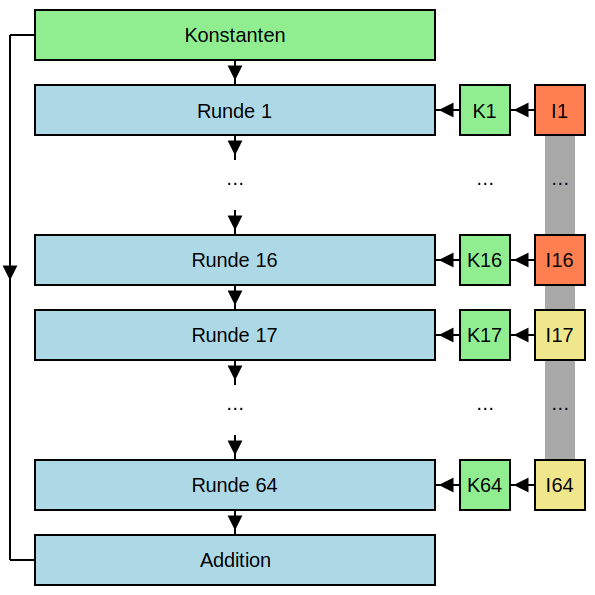
\includegraphics[scale=0.4]{images/sha256single}
  \caption{Schematische Darstellung einer einzelnen SHA-256-Berechnung}
  \label{fig:sha256single}
\end{figure}

Ist die Eingabe länger als 447 Bit, wird sie mit Hilfe des Paddings auf ein Vielfaches von 512 Bit erweitert. Der Algorithmus wird dann entsprechend oft ausgeführt,
wobei die acht 32 Bit breite Konstanten nur Eingang in die erste Berechnung finden. Das Ergebnis der ersten Berechnung dient dann als Startpunkt für die nächste
Berechnung. Dieses Schema ist in Abbildung \ref{fig:sha256multi} dargestellt.

\begin{figure}[!h]
  \centering
  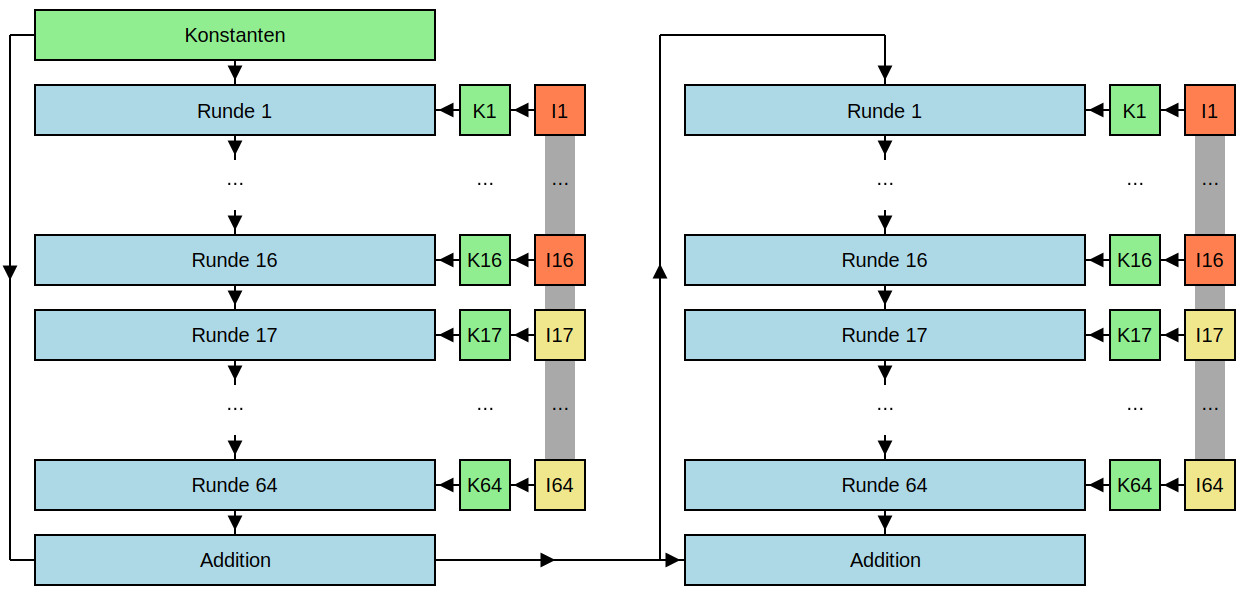
\includegraphics[scale=0.4]{images/sha256multi}
  \caption{Schematische Darstellung mehrerer SHA-256-Berechnungen}
  \label{fig:sha256multi}
\end{figure}

\section{Padding}
\label{sec:sha256:padding}

Um die Eingabe auf ein Vielfaches von 512 Bit zu erweitern, wird das Padding benötigt. Dabei wird ein einzelnes Bit mit dem Wert "`$1$"' an die Eingabe der Länge L gehängt.
Dann folgen K "`$0$"'en und abschließend ein 64 Bit Block, der die Länge L in binärer Repräsentation enthält. K ergibt sich dabei durch die Formel ( L + K ) mod 512 = 447.
Hier zeigt sich, dass bei einem K von 0 die Eingabe 447 Bit lang werden kann, bevor die Kompressionsfunktion weiteres Mal ausgeführt werden muss, weil ein zweiter 512 Bit Block
erzeugt wird.

\begin{figure}[!h]
  \centering
  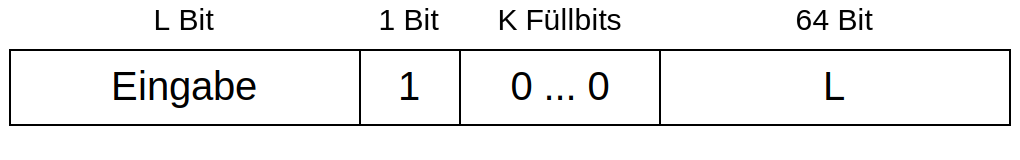
\includegraphics[scale=0.4]{images/sha256padding}
  \caption{Schematische Darstellung des Paddings}
  \label{fig:sha256padding}
\end{figure}
\section{Funktionen}
\label{sec:sha256:funktionen}

Die Funktion, die in \glos{sha256} am häufigsten verwendet wird, ist die modulare 32-Bit Addition (siehe Abschnitt \ref{sec:grundlagen_add}).
Darüber hinaus werden sowohl bei der Erweiterung der Eingabe als auch bei der Rundenfunktion einige Funktionen verwendet, die im folgendem erläutert werden.
Die Funktion "`Small Sigma"' wird bei der Erweiterung der Eingabe verwendet, während die Funktionen "`Choose"', "`Majority"' und "`Big Sigma"' in der Rundenfunktion
verwendet werden. Alle genannten Funktionen operieren auf einer Datenwortbreite von 32 Bit.

%Während die Aufgabe der Funktionen "`Choose"' und "`Majority"' die Konfusion ist, ist die Aufgabe der Sigma-Funktionen die Diffusion.
%Bei der Konfusion geht es darum, den Zusammenhang zwischen unterschiedlichen Werten zu verschleiern. Die Diffusion bewirkt den Einfluss
%eines Eingabebits auf viel Ausgabebits, um statistische Eigenschaften der Eingabe zu verstecken \cite[57]{crypto1}.

\subsection{Choose (CH)}
Choose steht für Wählen und beschreibt das Verhalten eines Multiplexers. Dabei bestimmt der Wert von x, ob y oder z das Ergebnis der Funktion bildet.
Durch die Datenwortbreite von 32 Bit, kommt es somit zu einer bitweisen Vermischung von y und z, die durch die Bits von x bestimmt wird. Dargestellt
ist die Funktion in Abbildung \ref{eq:ch}. Gemäß Standard \cite[10]{nist1804} führt das Ersetzen des XOR-Operators durch einen OR-Operator zu einem identischen Ergebnis.
\begin{figure}[!h]
  \begin{align}
  \text{CH}( x, y, z) &= (x~\wedge~y)~\oplus~( \neg~x~\wedge~z) \nonumber
  \end{align}
  \caption{Choose (CH)}
  \label{eq:ch}
\end{figure}

\subsection{Majority (MAJ)}
Majority steht für Mehrheit und bezieht sich auf die Anzahl der "`$1$"' und "`$0$"' Bits. Genau wie bei der Funktion "`Choose"' wird das Ergebnis aus drei Eingaben berechnet.
Es ergibt sich ein Ergebnis von "`$1$"', wenn mindestens zwei der Eingaben mit "`$1$"' belegt sind. Auch hier führt das Ersetzen des XOR-Operators durch einen OR-Operator zu
einem identischen Ergebnis.
\begin{figure}[!h]
  \begin{align}
  \text{MAJ}( x, y, z) &= (x~\wedge~y)~\oplus~(x~\wedge~z)~\oplus~(y~\wedge~z) \nonumber
  \end{align}
  \caption{Majority (MAJ)}
  \label{eq:maj}
\end{figure}

\subsection{Sigma (SIG)}
Die $\Sigma$-Funktionen werden in den \acr{rfc}s der \acr{ietf} mit SSIG und BSIG beschrieben, das vermutlich aus "`Small Sigma"' und "`Big Sigma"' abgeleitet wurde
um Sonderzeichen zu vermeiden. Die Sigma-Funktionen werden auch als Substitutions-Boxen (S-Boxen) bezeichnet \cite[1]{sha256analyse}. Jedes Bit der Ausgabe wir dabei
aus zwei bis drei Eingabebits berechnet. Da die Funktion 32 Bit auf 32 Bit abbildet, werden somit alle Eingabebits für zwei bis drei Ausgabebits verwendet.
Dargestellt sind alle vier Sigma-Funktionen in Abbildung \ref{eq:sig}.

Innerhalb der Funktionen wird die Rotation nach rechts (ROTR) und die Verschiebung nach rechts (SHR) verwendet. Im Unterschied zur Rotation, bei der die Bits,
die aus dem Register geschoben werden, auf der anderen Seite wieder eingefügt werden, werden die Bits bei der Verschiebung mit "`$0$"'en aufgefüllt.

Während bei den $\Sigma$-Funktionen konsequent drei Eingabebits mit dem XOR-Operator verknüpft werden um ein Ausgabebit zu berechnen, werden bei den $\sigma$-Funktionen
einige Bits durch die Verschiebung verworfen, was einem Angreifer die Analyse erschwert.

\begin{figure}[!h]
  \begin{align}
  \sigma_0(x) &= \text{ROTR}^{7}(x)~\oplus~\text{ROTR}^{18}(x)~\oplus~\text{SHR}^{3}(x) \nonumber\\
  \sigma_1(x) &= \text{ROTR}^{17}(x)~\oplus~\text{ROTR}^{19}(x)~\oplus~\text{SHR}^{10}(x) \nonumber\\
  \nonumber\\
  \Sigma_0(x) &= \text{ROTR}^{2}(x)~\oplus~\text{ROTR}^{13}(x)~\oplus~\text{ROTR}^{22}(x) \nonumber\\
  \Sigma_1(x) &= \text{ROTR}^{6}(x)~\oplus~\text{ROTR}^{11}(x)~\oplus~\text{ROTR}^{25}(x) \nonumber
  \end{align}
  \caption{Sigma (SIG)}
  \label{eq:sig}
\end{figure}
\section{Erweiterung der Eingabe}

\TODO{erledigen}

\begin{figure}[ht]
  \centering
  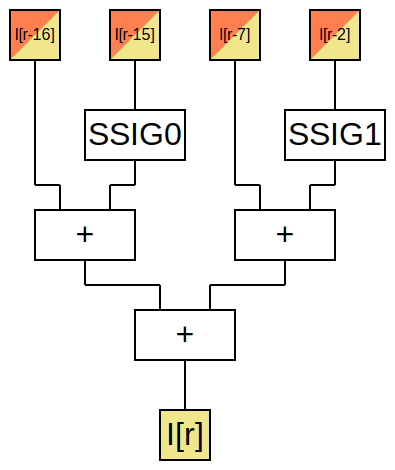
\includegraphics[scale=0.4]{images/sha256prep}
  \caption{Schematische Darstellung der Erweiterung}
  \label{fig:sha256prep}
\end{figure}
\section{Rundenfunktion}
\label{sec:sha256:runde}

Die Rundenfunktion ist in Abbildung \ref{fig:sha256core} dargestellt und ähnelt der eines doppelten Feistel-Netzwerks.
Es kommen sowohl die modulare 32-Bit Addition, die Choose- und Majority-Funktion, wie auch die beiden $\Sigma$-Funktionen zum Einsatz.
Bei einem Feistel-Netzwerk wird im allgemeinen ein Teil der Eingabe direkt in die Ausgabe kopiert während der andere
Teil unter Verwendung des ersten Teils verschlüsselt wird \cite[311]{crypto1}. Direkt kopiert werden sowohl A bis C
als auch E bis G. A' wird mit Hilfe von A bis C berechnet, während E' mit Hilfe von E bis G berechnet wird.
Als Schlüssel fließen D, H und I mit ein.

Initialisiert werden A bis H in der ersten Runde der ersten Kompression mit 8 Konstanten. Für die Konstanten mit 32 Bit Breite wurden laut
Standard \cite[10]{nist1804} die Quadratwurzel der ersten 8 Primzahlen herangezogen. Die ersten 32 Bit der Dezimalstellen jeder Quadratwurzel
ergeben die jeweilige Konstante. Mit Blick auf das Feistel-Netzwerk lassen sich diese Konstanten mit dem Klartext vergleichen, der mit der
Eingabe als Schlüssel zum Geheimtext entwickelt wird.

Enthalten ist in Abbildung \ref{fig:sha256core} auch die Addition der Rundenkonstante (K+). Für die Rundenkonstanten wurden laut Standard
\cite[10]{nist1804} die Kubikwurzel der ersten 64 Primzahlen herangezogen. Die ersten 32 Bit der Dezimalstellen jeder Kubikwurzel ergeben
die jeweilige Konstante. Die Addition der Konstanten bewirkt, dass der Einfluss der Eingabe sich in jeder Runde unterschiedlich auswirkt.

\begin{figure}[!h]
  \centering
  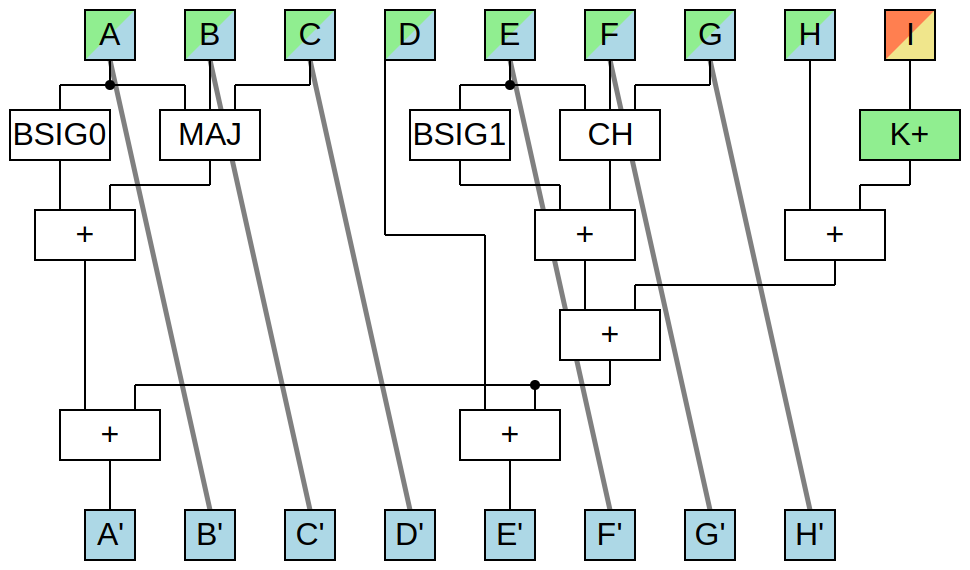
\includegraphics[scale=0.4]{images/sha256core}
  \caption{Schematische Darstellung einer SHA256-Runde}
  \label{fig:sha256core}
\end{figure}
\section{Analyse}
\label{sec:sha256:analyse}

In dieser Analyse geht es um eine oberflächliche Betrachtung der Rundenfunktion und des vollständigen Algorithmus.
Ziel ist es ein Verständnis dafür zu entwickeln, was eine Umkehrung der Berechnung verhindert und welche Berechnungen
notwendig wären, um bestimmte Ziele zu erreichen.

\subsection{Rundenfunktion}
In Abbildung \ref{fig:sha256coreA} ist noch einmal die Rundenfunktion mit einigen Markierungen dargestellt.
Bei dem Versuch, die Funktion umzukehren, ist sofort ersichtlich, dass A bis C und E bis G direkt übernommen werden können.

\begin{figure}[!h]
  \centering
  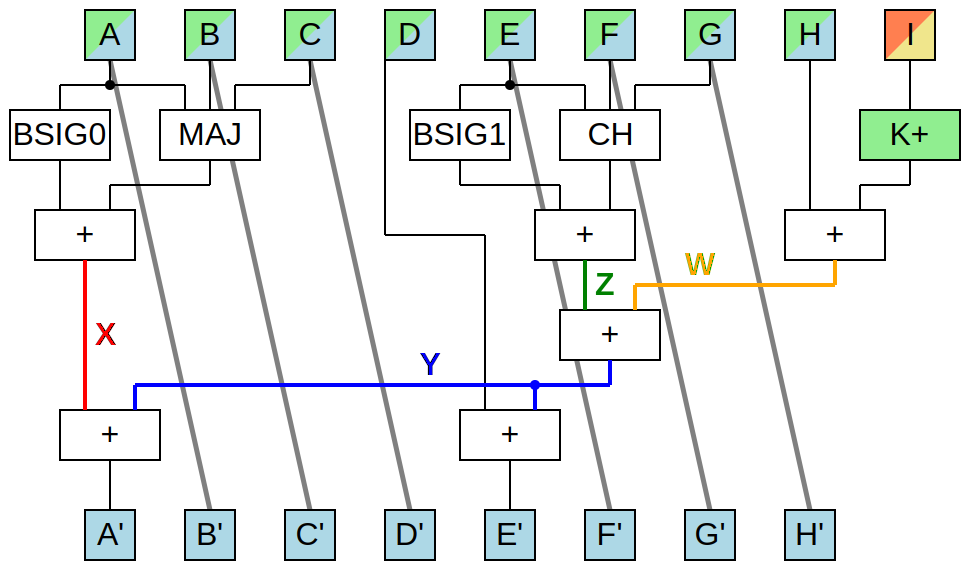
\includegraphics[scale=0.4]{images/sha256coreA}
  \caption{Analyse einer SHA256-Runde}
  \label{fig:sha256coreA}
\end{figure}

Dadurch lassen sich auch \textcolor{red}{\textbf{X}} und \textcolor{Strong Green}{\textbf{Z}} direkt berechnen.
Mit Hilfe von \textcolor{red}{\textbf{X}} lässt sich schließlich \textcolor{blue}{\textbf{Y}} berechnen, was zu D führt.
Formell ist dieser Zusammenhang in Abbildung \ref{eq:calcD} dargestellt.

\begin{figure}[!h]
  \begin{tabbing}
    XXXXXXXXXXXXXXXXXXXXX\=XX\=XX\=XXXXXX\=XXXX\=XX\=XX\=XXXXXXXX \kill
    \>A'\>=\>\textcolor{red}{\textbf{X}} + \textcolor{blue}{\textbf{Y}}\>$\Rightarrow$\>\textcolor{blue}{\textbf{Y}}\>=\>A' - \textcolor{red}{\textbf{X}}\\
    \>E'\>=\>D + \textcolor{blue}{\textbf{Y}}\>$\Rightarrow$\>\textcolor{blue}{\textbf{Y}}\>=\>E' - D\\
    \>~\\
    \>\>\>E' - D\>=\>A' - \textcolor{red}{\textbf{X}}\\
    \>\>\>-D    \>=\>A' - \textcolor{red}{\textbf{X}} - E'\\
    \>\>\>D     \>=\>\textcolor{red}{\textbf{X}} + E' - A'
  \end{tabbing}
  \caption{Berechnung von D}
  \label{eq:calcD}
\end{figure}

\subsection{Angriffsvektoren}

A bis H bei gegebenem Hash und Eingabe berechnen.\\
I jeweils bekannt jedoch fehlt A' bis H' da durch Addition mit Geheimnis "`maskiert"'.\\
Würde einen Angriff auf das Lösen einer einmalige Anwendung der 64 Runden bei beliebigen Eingabelängen reduzieren.
~\\
Eingabe bei gegebenem A bis H und Hash berechnen.\\
Problem ist es H/I zu bestimmen wie im Abschnitt vorher beschrieben\\
~\\
Geburtstagsparadoxon ausnutzen, ausgabe gleichsetzen und unterschied bei eingabe fordern